\documentclass[11pt,]{article}
\usepackage{lmodern}
\usepackage{amssymb,amsmath}
\usepackage{ifxetex,ifluatex}
\usepackage{fixltx2e} % provides \textsubscript
\ifnum 0\ifxetex 1\fi\ifluatex 1\fi=0 % if pdftex
  \usepackage[T1]{fontenc}
  \usepackage[utf8]{inputenc}
\else % if luatex or xelatex
  \ifxetex
    \usepackage{mathspec}
  \else
    \usepackage{fontspec}
  \fi
  \defaultfontfeatures{Ligatures=TeX,Scale=MatchLowercase}
    \setmainfont[]{Charis SIL}
\fi
% use upquote if available, for straight quotes in verbatim environments
\IfFileExists{upquote.sty}{\usepackage{upquote}}{}
% use microtype if available
\IfFileExists{microtype.sty}{%
\usepackage{microtype}
\UseMicrotypeSet[protrusion]{basicmath} % disable protrusion for tt fonts
}{}
\usepackage[margin=1in]{geometry}
\usepackage{hyperref}
\hypersetup{unicode=true,
            pdfborder={0 0 0},
            breaklinks=true}
\urlstyle{same}  % don't use monospace font for urls
\usepackage{natbib}
\bibliographystyle{unified.bst}
\usepackage{color}
\usepackage{fancyvrb}
\newcommand{\VerbBar}{|}
\newcommand{\VERB}{\Verb[commandchars=\\\{\}]}
\DefineVerbatimEnvironment{Highlighting}{Verbatim}{commandchars=\\\{\}}
% Add ',fontsize=\small' for more characters per line
\usepackage{framed}
\definecolor{shadecolor}{RGB}{248,248,248}
\newenvironment{Shaded}{\begin{snugshade}}{\end{snugshade}}
\newcommand{\AlertTok}[1]{\textcolor[rgb]{0.94,0.16,0.16}{#1}}
\newcommand{\AnnotationTok}[1]{\textcolor[rgb]{0.56,0.35,0.01}{\textbf{\textit{#1}}}}
\newcommand{\AttributeTok}[1]{\textcolor[rgb]{0.77,0.63,0.00}{#1}}
\newcommand{\BaseNTok}[1]{\textcolor[rgb]{0.00,0.00,0.81}{#1}}
\newcommand{\BuiltInTok}[1]{#1}
\newcommand{\CharTok}[1]{\textcolor[rgb]{0.31,0.60,0.02}{#1}}
\newcommand{\CommentTok}[1]{\textcolor[rgb]{0.56,0.35,0.01}{\textit{#1}}}
\newcommand{\CommentVarTok}[1]{\textcolor[rgb]{0.56,0.35,0.01}{\textbf{\textit{#1}}}}
\newcommand{\ConstantTok}[1]{\textcolor[rgb]{0.00,0.00,0.00}{#1}}
\newcommand{\ControlFlowTok}[1]{\textcolor[rgb]{0.13,0.29,0.53}{\textbf{#1}}}
\newcommand{\DataTypeTok}[1]{\textcolor[rgb]{0.13,0.29,0.53}{#1}}
\newcommand{\DecValTok}[1]{\textcolor[rgb]{0.00,0.00,0.81}{#1}}
\newcommand{\DocumentationTok}[1]{\textcolor[rgb]{0.56,0.35,0.01}{\textbf{\textit{#1}}}}
\newcommand{\ErrorTok}[1]{\textcolor[rgb]{0.64,0.00,0.00}{\textbf{#1}}}
\newcommand{\ExtensionTok}[1]{#1}
\newcommand{\FloatTok}[1]{\textcolor[rgb]{0.00,0.00,0.81}{#1}}
\newcommand{\FunctionTok}[1]{\textcolor[rgb]{0.00,0.00,0.00}{#1}}
\newcommand{\ImportTok}[1]{#1}
\newcommand{\InformationTok}[1]{\textcolor[rgb]{0.56,0.35,0.01}{\textbf{\textit{#1}}}}
\newcommand{\KeywordTok}[1]{\textcolor[rgb]{0.13,0.29,0.53}{\textbf{#1}}}
\newcommand{\NormalTok}[1]{#1}
\newcommand{\OperatorTok}[1]{\textcolor[rgb]{0.81,0.36,0.00}{\textbf{#1}}}
\newcommand{\OtherTok}[1]{\textcolor[rgb]{0.56,0.35,0.01}{#1}}
\newcommand{\PreprocessorTok}[1]{\textcolor[rgb]{0.56,0.35,0.01}{\textit{#1}}}
\newcommand{\RegionMarkerTok}[1]{#1}
\newcommand{\SpecialCharTok}[1]{\textcolor[rgb]{0.00,0.00,0.00}{#1}}
\newcommand{\SpecialStringTok}[1]{\textcolor[rgb]{0.31,0.60,0.02}{#1}}
\newcommand{\StringTok}[1]{\textcolor[rgb]{0.31,0.60,0.02}{#1}}
\newcommand{\VariableTok}[1]{\textcolor[rgb]{0.00,0.00,0.00}{#1}}
\newcommand{\VerbatimStringTok}[1]{\textcolor[rgb]{0.31,0.60,0.02}{#1}}
\newcommand{\WarningTok}[1]{\textcolor[rgb]{0.56,0.35,0.01}{\textbf{\textit{#1}}}}
\usepackage{graphicx,grffile}
\makeatletter
\def\maxwidth{\ifdim\Gin@nat@width>\linewidth\linewidth\else\Gin@nat@width\fi}
\def\maxheight{\ifdim\Gin@nat@height>\textheight\textheight\else\Gin@nat@height\fi}
\makeatother
% Scale images if necessary, so that they will not overflow the page
% margins by default, and it is still possible to overwrite the defaults
% using explicit options in \includegraphics[width, height, ...]{}
\setkeys{Gin}{width=\maxwidth,height=\maxheight,keepaspectratio}
\setlength{\emergencystretch}{3em}  % prevent overfull lines
\providecommand{\tightlist}{%
  \setlength{\itemsep}{0pt}\setlength{\parskip}{0pt}}
\setcounter{secnumdepth}{5}
% Redefines (sub)paragraphs to behave more like sections
\ifx\paragraph\undefined\else
\let\oldparagraph\paragraph
\renewcommand{\paragraph}[1]{\oldparagraph{#1}\mbox{}}
\fi
\ifx\subparagraph\undefined\else
\let\oldsubparagraph\subparagraph
\renewcommand{\subparagraph}[1]{\oldsubparagraph{#1}\mbox{}}
\fi

%%% Use protect on footnotes to avoid problems with footnotes in titles
\let\rmarkdownfootnote\footnote%
\def\footnote{\protect\rmarkdownfootnote}

%%% Change title format to be more compact
\usepackage{titling}

% Create subtitle command for use in maketitle
\providecommand{\subtitle}[1]{
  \posttitle{
    \begin{center}\large#1\end{center}
    }
}

\setlength{\droptitle}{-2em}

  \title{}
    \pretitle{\vspace{\droptitle}}
  \posttitle{}
    \author{}
    \preauthor{}\postauthor{}
    \date{}
    \predate{}\postdate{}
  
\usepackage{cleveref}
\usepackage{lineno}
\linenumbers

\begin{document}

\large

TITLE: Assessing mid-saggital tongue contours in polar coordinates using
generalised additive (mixed) models

\vspace{1cm}

AUTHOR: Stefano Coretta

\vspace{1cm}

AFFILIATION: Linguistics and English Language, University of Manchester,
Oxford Road, Manchester, M13 9PL, United Kingdom

\vspace{1cm}

EMAIL ADDRESS:
\href{mailto:stefano.coretta@manchester.ac.uk}{\nolinkurl{stefano.coretta@manchester.ac.uk}}

\normalsize

\pagebreak

\begin{abstract}
Statistical modelling of whole tongue contours has been mostly dominated by the use of Smoothing Splines Analysis of Variance (SSANOVA), although the quantitative analysis of UTI data remains a challenge.
Recently, a variety of research disciplines witnessed an increased use of Generalised Additive Models (GAMs) and their mixed-effects counterpart.
This family of models is a highly flexible solution which extends standard generalised linear mixed regressions to model non-linear effects.
This paper offers a review of GAMs fitted to tongue contours in polar coordinates, as an alternative to polar SSANOVA, given the increasing popularity of these models among linguists.
Polar GAMs fitting, significance testing, and model plotting are illustrated by means of an example study that compares tongue contours of voiceless and voiced stops of 12 speakers of Italian and Polish.
A brief tutorial illustrates fitting and plotting of polar GAMs with the R package rticulate.
The series of polar GAMs indicates a high degree of idiosyncrasy in tongue root position in voiceless and voiced stops, within and across speakers.
Limitations of the current implementation of polar GAMs (such as across-speaker normalisation) and future directions are also briefly discussed.
\end{abstract}

\textbf{Keywords}: ultrasound tongue imaging, generalised additive
models, tongue root

\hypertarget{introduction}{%
\section{Introduction}\label{introduction}}

Since the publication of the seminal paper by \citet{davidson2006},
statistical modelling of whole tongue contours obtained with ultrasound
imaging has been dominated by the use of Smoothing Splines Analysis of
Variance (SSANOVA, \citealt{gu2013}). These models have greatly advanced
our understanding of tongue articulation and speech modelling. On the
other hand, Generalised Additive Models (GAMs) and their mixed-effects
counterpart (GAMMs, \citealt{wood2006}) are increasingly adopted in
linguistics as a means to model complex data. This paper introduces an
implementation of GAMs fitted to tongue contours using a polar
coordinate system. The implementation of polar GAMs is illustrated with
ultrasound tongue imaging data of an example study that compares
voiceless and voiced stops. A brief tutorial shows how to fit polar GAMs
with the R package rticulate, developed to facilitate the fitting
procedure. Among the advantages of polar GAMs over the current
implementation of polar tongue SSANOVA is the possibility of modelling
the effect of multiple predictors and that of controlling for
autocorrelation in the residuals with the inclusion of autoregressive
models.

\hypertarget{ultrasound-tongue-imaging}{%
\subsection{Ultrasound tongue imaging}\label{ultrasound-tongue-imaging}}

Ultrasound imaging is a non-invasive technique for obtaining an image of
internal organs and other body tissues. 2D ultrasound imaging has been
successfully used for imaging sections of the tongue surface (for a
review, see \citealt{gick2002} and \citealt{lulich2018}). An image of
the (2D) tongue surface can be obtained by placing the transducer in
contact with the sub-mental triangle (the area under the chin), aligned
either with the mid-sagittal or the coronal plane. The ultrasonic waves
propagate from the transducer in a radial fashion through the aperture
of the mandible and get reflected when they hit the air above the tongue
surface. This `echo' is captured by the transducer and translated into
an image like the one shown in \Cref{f:uti} (for a technical
description, see \citealt{stone2005}).

\begin{figure}
  \centering
  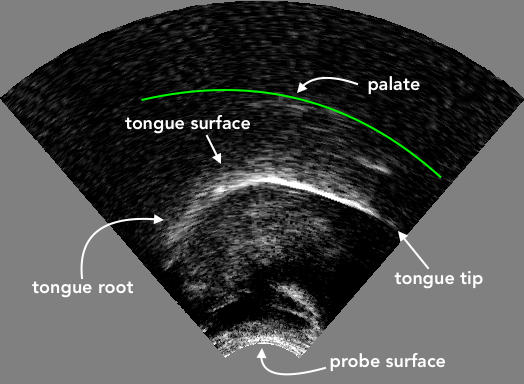
\includegraphics{./img/Figure01-uti.png}
  \caption{An ultrasound image showing a mid-sagittal view of the tongue. The white curved stripe in the image indicates where the ultrasonic waves have been reflected by the air above the tongue. The tongue surface corresponds to the lower edge of the white stripe. In this image, the tongue tip is located on the right. The green curve approximates the location of the palate.}
  \label{f:uti}
\end{figure}

\hypertarget{generalised-additive-models}{%
\subsection{Generalised Additive
models}\label{generalised-additive-models}}

Generalised additive models, or GAMs, are a more general form of
non-parametric modelling that allows fitting non-linear as well as
linear effects, and combine properties of linear and additive modelling
\citep{hastie1986}. GAMs are built with smoothing splines (like SSANOVA,
see \citealt{helwig2016}), which are defined piecewise with a set (the
\emph{basis}) of polynomial functions (the \emph{basis functions}). When
fitting GAMs, the smoothing splines try to maximise the fit to the data
while being constrained by a smoothing penalty (usually estimated from
the data itself). Such penalisation constitutes a guard against
overfitting. GAMs are thus powerful and flexible models that can deal
with non-linear data efficiently.

Moreover, GAMs have a mixed-effect counterpart, Generalised Additive
Mixed Models (GAMMs), in which random effects can be included (for a
technical introduction to GAM(M)s, see \citealt{zuur2012} and
\citealt{wood2017}). GAMs can offer relief from issues of
autocorrelation between points of a tongue contour (given that points
close to each other are not independent from one another). For example,
GAMs can fit separate smooths to individual contours, or a first-order
autoregression model can be included which tries to account for the
autocorrelation between each point in the contour and the one following
it. Tongue contours obtained from ultrasound imaging lend themselves to
be efficiently modelled using GAM(M)s.

\hypertarget{polar-coordinates}{%
\subsection{Polar coordinates}\label{polar-coordinates}}

\citet{mielke2015} and \citet{heyne2015a, heyne2015} have shown that
using polar coordinates of tongue contours rather than cartesian
coordinates brings several benefits, among which reduced variance at the
edges of the tongue contour. Points in a polar coordinate system are
defined by pairs of radial and angular values. A point is described by a
radius, which corresponds to the radial distance from the origin, and by
the angle from a reference radius. Tongue contours, due to their shape,
tend to have increasing slope at the left and right edges, in certain
cases tending to become almost completely vertical. The verticality of
the contours has the effect of increasing the variance of the fitted
contours (and hence the confidence intervals), and in some cases it can
even generate uninterpretable curves.

This issue is illustrated in \Cref{f:Figure02}. The \emph{x} and
\emph{y} axes are the \emph{x} and \emph{y} cartesian coordinates in
millimeters. The plot shows LOESS smooths superimposed on the points of
the individual tongue contours of an Italian speaker (IT01, see
\Cref{s:data}). These contours refer to the mid-sagittal shape of the
tongue during the closure of four consonants (/t, d, k, g/) preceded by
one of three vowels (/a, o, u/). The tip of the tongue is on the
right-end side of each panel. Focussing on the smooths, it can be
noticed that the smooths in the contexts of the vowel /u/ diverge
substantially from the true contours (as inferred by the points). In the
contexts of velar consonants and the other two vowels, the back/root of
the tongue is somewhat flattened out relative to the actual contours.
These smoothing artefacts arise because, especially at the left-edge of
these particular contours, the slope of the curve increases in such a
way that the curve bends under itself (see for example the context /ug/,
when \emph{x} is between -30 and -20). Since those points on the bend
share the same \emph{x} value, the smooth just averages across the
\emph{y} values of those points. \Cref{f:Figure03} shows a more
appropriate (artefact-free) way of representing individual tongue
contours. In these plots, the points of each contour are connected
sequentially by a line, rather than smoothed over. The parts in which
the contours bend over themselves are kept as such and visualised
correctly.

\begin{figure}

{\centering 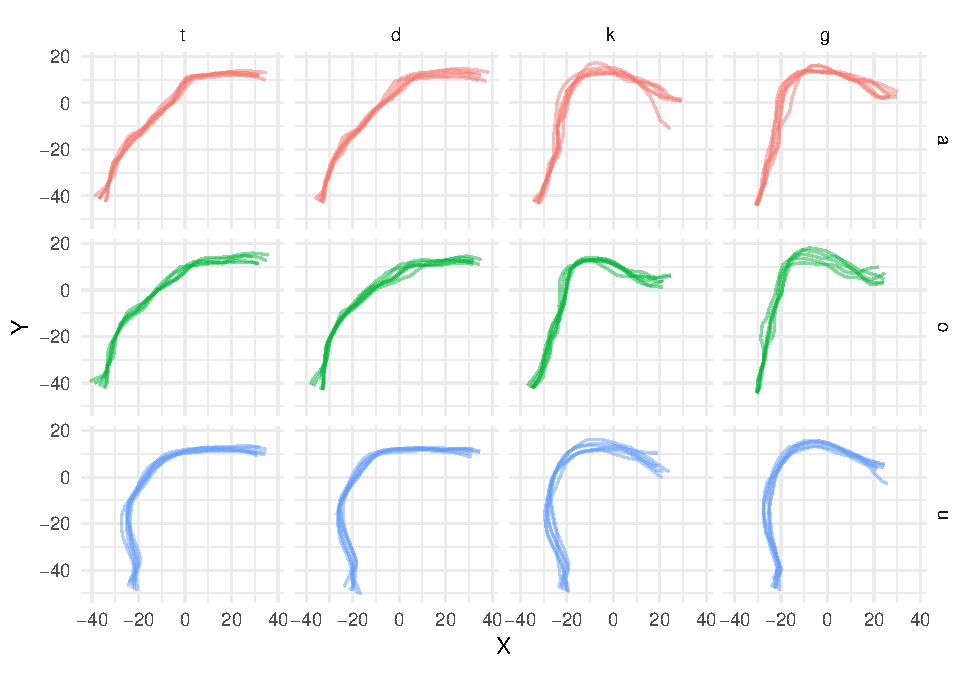
\includegraphics[width=\linewidth]{2018-polar-gam_files/figure-latex/Figure02} 

}

\caption{Estimated tongue contours of IT01 depending on C2 place, vowel and C2 voicing.}\label{f:Figure02}
\end{figure}

\begin{figure}

{\centering 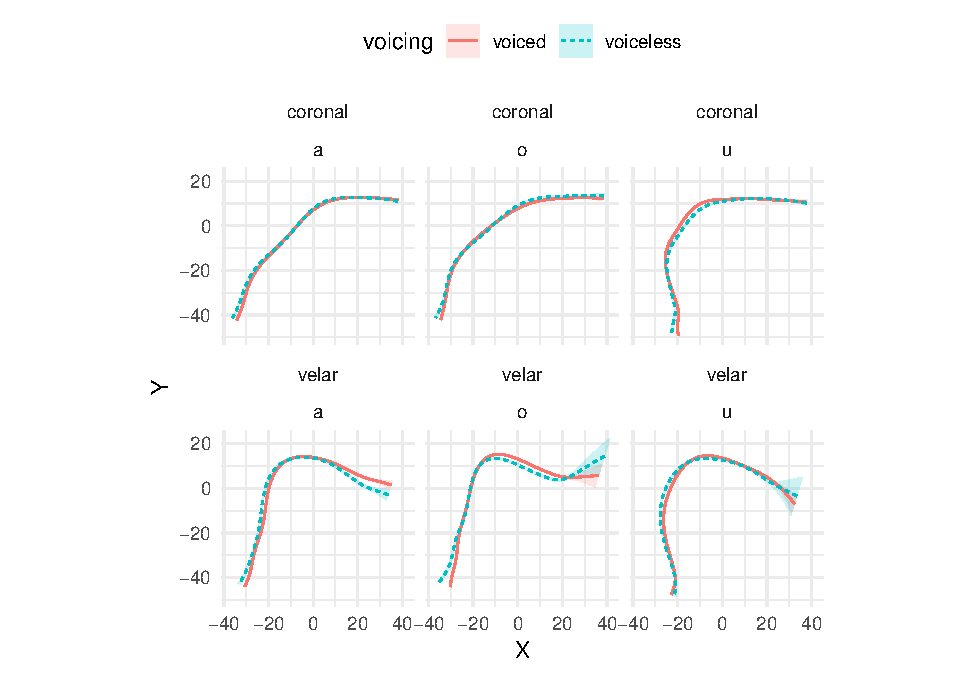
\includegraphics[width=\linewidth]{2018-polar-gam_files/figure-latex/Figure03} 

}

\caption{Estimated tongue contours of IT01 depending on C2 place, vowel and C2 voicing.}\label{f:Figure03}
\end{figure}

These figures illustrate that using cartesian coordinates for modelling
tongue contours can introduce smoothing artefacts which can in turn
negatively affect the model output. When tongue contours are expressed
with polar coordinates, on the other hand, the variance is reduced and
the fitted contours generally reflect more closely the underlying tongue
shape. Mielke has implemented a series of R \citep{r-core-team2018}
functions for fitting polar SSANOVAs to tongue contours
(\url{http://phon.chass.ncsu.edu/manual/tongue_ssanova.r}). While model
fitting is achieved using polar coordinates, plotting is done by
reconverting the coordinates to a cartesian system. This same procedure
is used in the polar GAM modelling presented here.

\hypertarget{polar-gamms}{%
\section{Polar GAM(M)s}\label{polar-gamms}}

GAMs fitted to tongue contours in polar coordinates are introduced here.
A polar GAM is constructed as follows. The outcome variable of the model
are the radial coordinates, while a smooth term over the angular
coordinates is the predictor which takes care of modelling the curved
shape of the contour. Other predictors, such as consonant or vowel type,
speech rate, or random effects, can also be included. The model returns
fitted smooths in polar coordinates. The predicted polar coordinates of
the smooths can be derived from the model and converted into a cartesian
coordinate system (centred on the origin of the polar system) for
plotting. A simple example with data from one speaker will illustrate
how to fit polar GAMs with the R package rticulate. The following
section gives information on the ultrasonic system used for data
collection and on how the data has been processed, before moving onto
model fitting itself.

\hypertarget{data-collection-and-processing}{%
\subsection{Data collection and
processing}\label{data-collection-and-processing}}

\label{s:data}

Synchronised audio and ultrasound tongue imaging data have been recorded
from 11 speakers of Italian and 6 speakers of Polish while reading a
series of controlled sentences. An Articulate Instruments Ltd™ set-up
was used for this study. The ultrasonic data was collected through a
TELEMED Echo Blaster 128 unit with a TELEMED C3.5/20/128Z-3 ultrasonic
transducer (20mm radius, 2-4 MHz). A synchronisation unit (P-Stretch)
was plugged into the Echo Blaster unit and used for automatic
audio/ultrasound synchronisation. A FocusRight Scarlett Solo
pre-amplifier and a Movo LV4-O2 Lavalier microphone were used for audio
recording. The acquisition of the ultrasonic and audio signals was
achieved with the software Articulate Assistant Advanced (AAA, v2.17.2)
running on a Hawlett-Packard ProBook 6750b laptop with Microsoft Windows
7. Stabilisation of the ultrasonic transducer was ensured by using the
metallic headset produced by Articulate Instruments Ltd™
(\citeyear{articulate2008}).

Before the reading task, the participant's occlusal plane was obtained
using a bite plate \citep{scobbie2011}. The participants read nonce
words embedded in the frame sentence \emph{Dico \_\_ lentamente} `I say
\_\_ slowly' (Italian) and \emph{Mówię \_\_ teraz} `I say \_\_ now'
(Polish). The words follow the structure
C\textsubscript{1}V́\textsubscript{1}C\textsubscript{2}V\textsubscript{2},
where C\textsubscript{1} = /p/, V\textsubscript{1} = /a, o, u/,
C\textsubscript{2} = /t, d, k, g/, and V\textsubscript{2} =
V\textsubscript{1}. Each speaker repeated the stimuli six times.

Spline curves were fitted to the visible tongue contours using the AAA
automatic tracking function. Manual correction was applied in those
cases that showed clear tracking errors. The time of maximum tongue
displacement within consonant closure was then calculated in AAA
following the method in \citet{strycharczuk2015}. A fan-like frame
consisting of 42 equidistant radial lines was used as the coordinate
system. The origin of the 42 fan-lines coincides with the centre of the
ultrasonic probe, such that each fan-line is parallel to the direction
of the ultrasonic signal. Tongue displacement was thus calculated as the
displacement of the fitted splines along the fan-line vectors. The time
of maximum tongue displacement was the time of greater displacement
along the fan-line vector with the greatest standard deviation. The
vector standard deviation search area was restricted to the portion of
the contour corresponding to the tongue tip for coronal consonants, and
to the portion corresponding to the tongue dorsum for velar consonants.

The cartesian coordinates of the tongue contours were extracted from the
ultrasonic data at the time of maximum tongue displacement (always
within C2 closure). The contours were subsequently normalised within
speaker by applying offsetting and rotation relative to the
participant's occlusal plane \citep{scobbie2011}. Each participants'
dataset is thus constituted by \emph{x} and \emph{y} coordinates of the
tongue contours that define respectively the horizontal and vertical
axes. The horizontal plane is parallel to the speaker's occlusal plane.

\hypertarget{fitting-a-polar-gam}{%
\subsection{Fitting a polar GAM}\label{fitting-a-polar-gam}}

GAMs can be fitted in R with the \texttt{gam()} function from package
mgcv \citep{wood2011, wood2017}. \texttt{bam()} is a more efficient
function when the dataset has several hundreds observations. The package
rticulate has been developed as a wrapper of the \texttt{bam()} function
to be used with tongue contours. The special function
\texttt{polar\_gam()} can fit a variety of GAM models to tongue contours
coordinates, using the same syntax of mgcv. The function accepts tongue
contours either in cartesian or polar coordinates. In the first case,
the coordinates can be transformed into polar before fitting. If the
data is in the AAA fan-like coordinate system, the origin is
automatically estimated with the method in \citet{heyne2015a}. If the
data is not exported from AAA, the user can specify the known
coordinates of the probe origin. The function
\texttt{plot\_polar\_smooths()}, used for plotting the estimated
contours, converts the coordinates back into cartesian using the same
origin as with GAM fitting.

A GAM in R can be specified with a formula that uses the same syntax of
lme4, a commonly used package for linear mixed-effects models
\citep{bates2015}. The mgcv package allows to specify smoothing spline
terms with the function \texttt{s()}. This function takes the term along
which a spline is created (for example, time in a time series, or
\emph{x}-coordinates in a cartesian system). Among the arguments of
\texttt{s()}, the user can select the type of spline (the \texttt{bs}
argument) and the grouping factor used for comparison (the \texttt{by}
argument). For a more in-depth introduction to GAMs in R for
linguistics, see \citet{soskuthy2017} and \citet{wieling2017}.

As means of illustration, the following paragraphs will show how to fit
a polar GAM with data from one of the Italian speakers. Due to
differences in the placement of the probe and in the speakers' anatomy,
different portions of the tongue are likely to be imaged across
speakers, so that scaling might not be possible (or wise). For this
reason, it is recommended to fit separate models for each participant,
rather than aggregate all of the data in a single model.

We can start from a simple model in which we test the effect of C2
place, vowel, and voicing on tongue contours. \texttt{vc\_voicing} is an
ordered factor that specifies the combination of C2 place, vowel, and
voicing. Modelling different contours for each combination of the three
predictors can be achieved by using \texttt{vc\_voicing} with the
\texttt{by} argument of the difference smooth, and by including
\texttt{vc\_voicing} as a parametric term. The following code fits the
specified model to the contour data of IT01. When running the code, the
coordinates of the estimated origin used for the conversion to polar
coordinates are returned. The model is fitted by Maximum Likelihood (ML)
here to allow model comparison below.

\begin{Shaded}
\begin{Highlighting}[]
\NormalTok{it01_gam <-}\StringTok{ }\KeywordTok{polar_gam}\NormalTok{(}
\NormalTok{  Y }\OperatorTok{~}
\StringTok{    }\NormalTok{vc_voicing }\OperatorTok{+}\StringTok{            }\CommentTok{# parametric term}
\StringTok{    }\KeywordTok{s}\NormalTok{(X) }\OperatorTok{+}\StringTok{                  }\CommentTok{# reference smooth}
\StringTok{    }\KeywordTok{s}\NormalTok{(X, }\DataTypeTok{by =}\NormalTok{ vc_voicing),  }\CommentTok{# difference smooth}
  \DataTypeTok{data =}\NormalTok{ tongue_it01,}
  \DataTypeTok{method =} \StringTok{"ML"}
\NormalTok{)}
\end{Highlighting}
\end{Shaded}

\begin{verbatim}
## The origin is x = 14.3901068810439, y = -65.2314851170583.
\end{verbatim}

The function \texttt{plot\_polar\_smooths()} can be used to plot the
estimated contours. The shaded areas around the estimated contours are
95\% confidence intervals. Note that, differently from SSANOVA,
statistical significance can't be assessed from the overlapping (or lack
thereof) of the confidence intervals. The output of
\texttt{plot\_polar\_smooths()} is shown in \Cref{f:Figure04}. For more
details on fitting and plotting more complex models (for example models
with multiple predictors or tensor product smooths), see the package
vignette \texttt{polar-gams} (accessible with
\texttt{vignette("polar-gams",\ package\ =\ "rticulate")}).

\begin{Shaded}
\begin{Highlighting}[]
\KeywordTok{plot_polar_smooths}\NormalTok{(}
\NormalTok{  it01_gam,}
\NormalTok{  X,}
\NormalTok{  voicing,}
  \DataTypeTok{facet_terms =}\NormalTok{ c2_place }\OperatorTok{+}\StringTok{ }\NormalTok{vowel,}
  \CommentTok{# the following splits the factor interaction into the individual terms,}
  \CommentTok{# so that they can be called in the plotting arguments}
  \DataTypeTok{split =} \KeywordTok{list}\NormalTok{(}\DataTypeTok{vc_voicing =} \KeywordTok{c}\NormalTok{(}\StringTok{"vowel"}\NormalTok{, }\StringTok{"c2_place"}\NormalTok{, }\StringTok{"voicing"}\NormalTok{))}
\NormalTok{) }\OperatorTok{+}
\StringTok{  }\KeywordTok{coord_fixed}\NormalTok{() }\OperatorTok{+}
\StringTok{  }\KeywordTok{theme}\NormalTok{(}\DataTypeTok{legend.position =} \StringTok{"top"}\NormalTok{)}
\end{Highlighting}
\end{Shaded}

\begin{figure}

{\centering 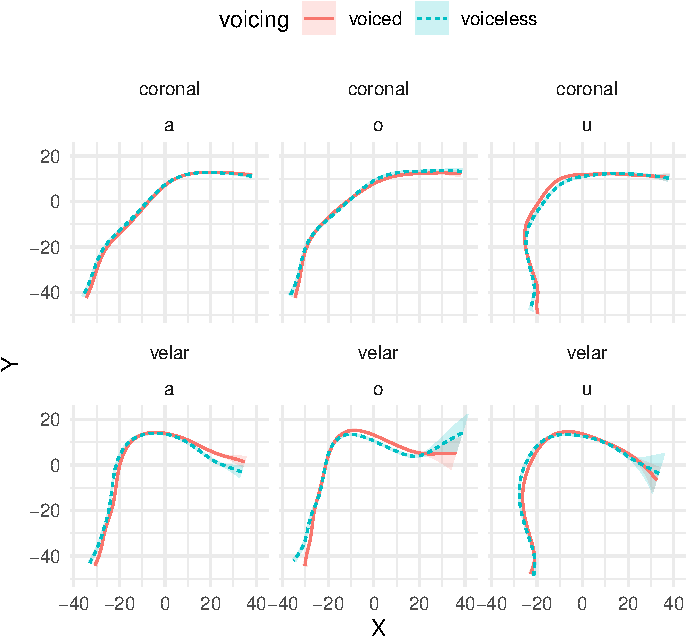
\includegraphics[width=\linewidth]{2018-polar-gam_files/figure-latex/Figure04} 

}

\caption{Estimated tongue contours of IT01 depending on C2 place, vowel and C2 voicing.}\label{f:Figure04}
\end{figure}

One way to assess significance of model terms is to compare the ML score
of the full model against one without the relevant predictor, using the
function \texttt{compareML()} from the itsadug package
\citep{van-rij2017}. Both the parametric term and the difference smooth
need to be removed in the null model.

\begin{Shaded}
\begin{Highlighting}[]
\NormalTok{it01_gam_}\DecValTok{0}\NormalTok{ <-}\StringTok{ }\KeywordTok{polar_gam}\NormalTok{(}
\NormalTok{  Y }\OperatorTok{~}
\StringTok{    }\CommentTok{# vc_voicing +            # remove parametric term}
\StringTok{    }\KeywordTok{s}\NormalTok{(X),                     }\CommentTok{# keep reference smooth}
    \CommentTok{# s(X, by = vc_voicing),  # remove difference smooth}
  \DataTypeTok{data =}\NormalTok{ tongue_it01,}
  \DataTypeTok{method =} \StringTok{"ML"}
\NormalTok{)}
\end{Highlighting}
\end{Shaded}

\begin{verbatim}
## The origin is x = 14.3901068810439, y = -65.2314851170583.
\end{verbatim}

\begin{Shaded}
\begin{Highlighting}[]
\KeywordTok{compareML}\NormalTok{(it01_gam_}\DecValTok{0}\NormalTok{, it01_gam)}
\end{Highlighting}
\end{Shaded}

\begin{verbatim}
## it01_gam_0: Y ~ s(X)
## 
## it01_gam: Y ~ vc_voicing + s(X) + s(X, by = vc_voicing)
## 
## Chi-square test of ML scores
## -----
##        Model    Score Edf Difference     Df  p.value Sig.
## 1 it01_gam_0 7085.662   3                                
## 2   it01_gam 4417.403  36   2668.260 33.000  < 2e-16  ***
## 
## AIC difference: 5603.15, model it01_gam has lower AIC.
\end{verbatim}

To check which part of the contour differs among conditions, the method
recommended in \citet{soskuthy2017} is to plot the difference smooth and
check the confidence interval. The parts of the confidence interval that
don't include 0 indicate that the difference between contours in that
part is significant. \Cref{f:Figure05} illustrates the use of difference
smooths with the difference smooths of voiceless vs.~voiced coronal
stops when the vocalic context is /a/ or /u/. As per usual, the tongue
tip is on the right-end side of each plot. The difference smooths
indicate that there is a significant difference along the posterior part
of the tongue (the root and dorsum). Based on the predicted smooths sown
in \Cref{f:Figure04}, we can argue that, in the context of coronal
consonants, the root is more advanced in voiced relative to voiceless
stops (when the vowel is either /a/ or /u/), and that the dorsum is also
somewhat retracted in voiced stops if the vowel is /u/.

\begin{figure}

{\centering 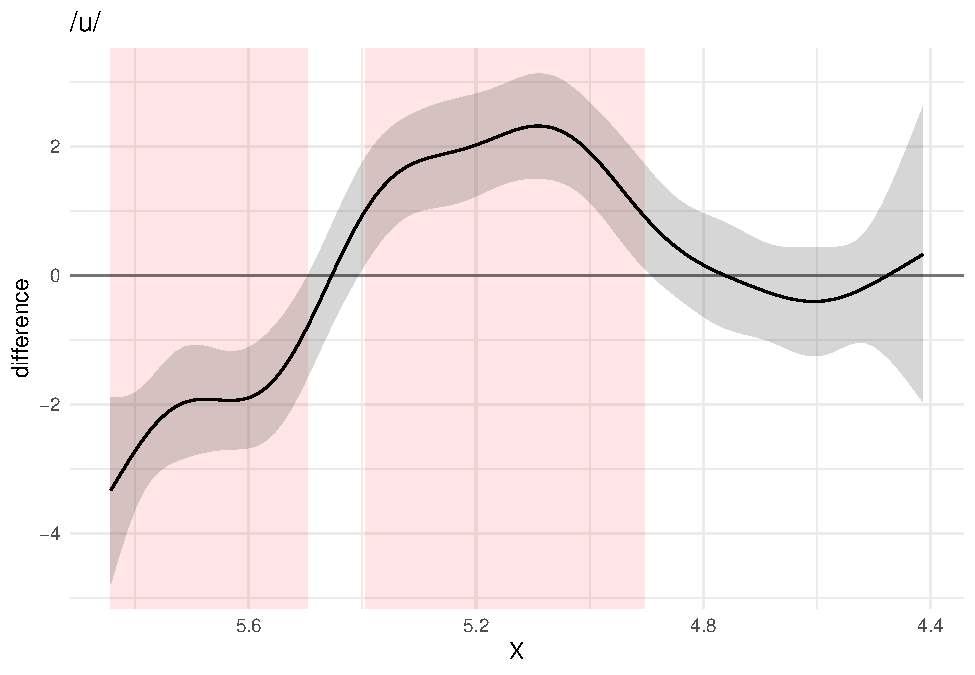
\includegraphics[width=.7\linewidth,height=5cm]{2018-polar-gam_files/figure-latex/Figure05} 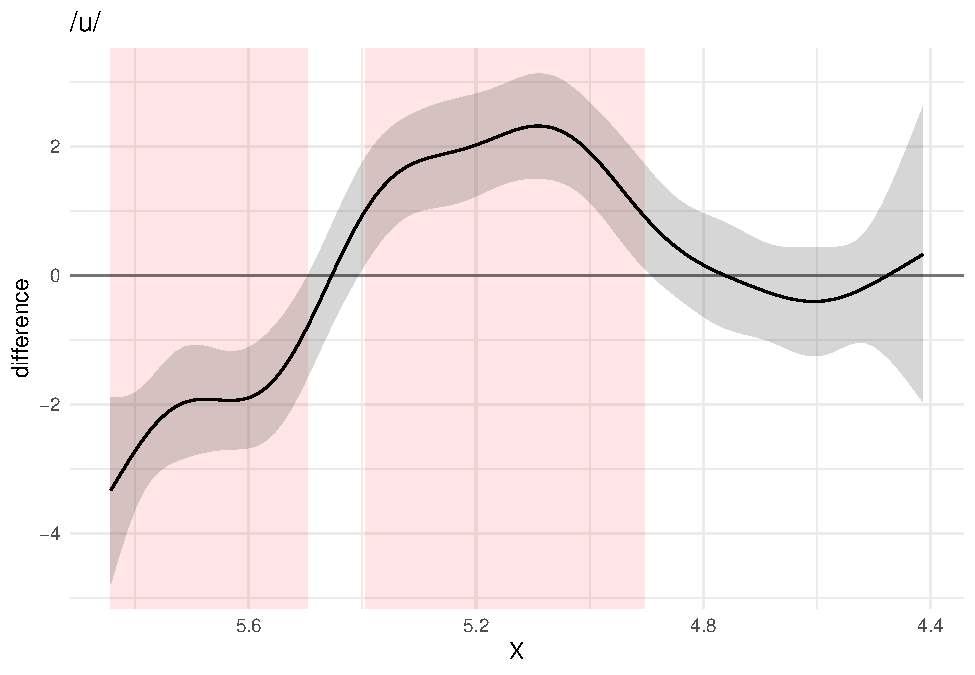
\includegraphics[width=.7\linewidth,height=5cm]{2018-polar-gam_files/figure-latex/Figure05} 

}

\caption{Difference smooth of voiceless vs. voiced stops in the context of /a/ (left) and /u/ (right).}\label{f:Figure05}
\end{figure}

As mentioned in the introduction, autocorrelation in the data can
produce unwanted patterns in the residuals, which in turn can affect the
estimated smooths (and falsely increase certainty about them). A
first-order autoregressive (AR1) model can be included to reduce
autocorrelation at lag 1. \Cref{f:Figure06} show the autocorrelations in
the residuals without (left) and with (right) an AR1 model. The GAM
model with the AR1 correction has lower autocorrelation values. In this
case, it is thus advisable to perform ML comparison and smooths plotting
with models in which an AR1 model has been included. For a more in-depth
treatment of issues related to autocorrelation, see
\citet{soskuthy2017}.

\begin{figure}

{\centering 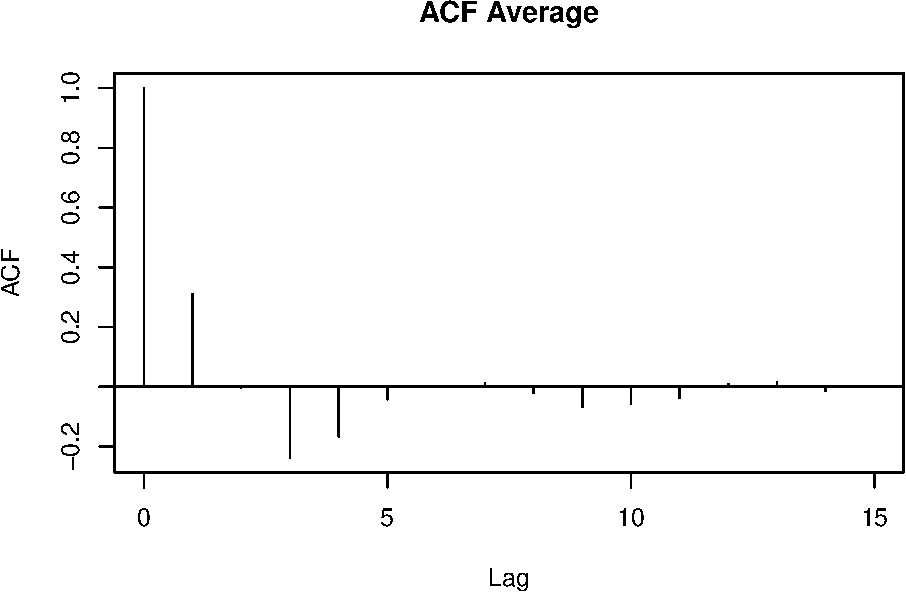
\includegraphics[width=.7\linewidth,height=5cm]{2018-polar-gam_files/figure-latex/Figure06} 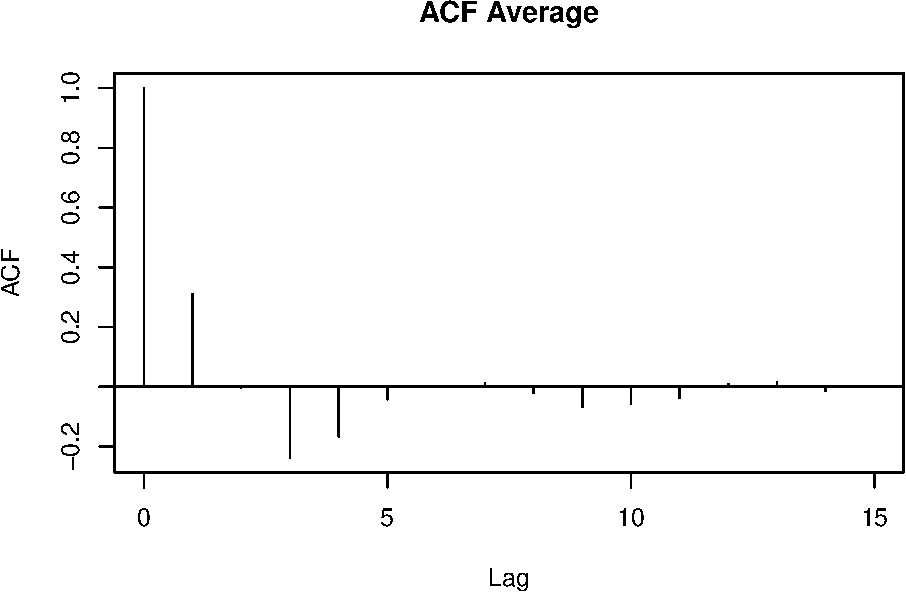
\includegraphics[width=.7\linewidth,height=5cm]{2018-polar-gam_files/figure-latex/Figure06} 

}

\caption{Autocorrelation plots of a model fitted without (left) and with (right) a first-order autoregressive model (AR1).}\label{f:Figure06}
\end{figure}

\hypertarget{comparing-tongue-root-position-in-voiceless-and-voiced-stops}{%
\section{Comparing tongue root position in voiceless and voiced
stops}\label{comparing-tongue-root-position-in-voiceless-and-voiced-stops}}

Tongue root advancement is a well-known mechanism employed to keep
intra-oral pressure below the threshold required for voicing
\citep{ohala2011, kent1969, perkell1969, westbury1983, ahn2018}. Among
the languages reported to show tongue root position differences between
phonation categories in stops there are English
\citep{westbury1983, ahn2018}, Brazilian Portuguese \citep{ahn2018}, and
Hindi \citep{ahn2016a}. Tongue root advancement is one of several
mechanisms employed by speakers to enlarge the oral cavity during the
production of a stop closure. The decrease in pressure that follows from
such expansion ensures that voicing can be maintained during the
closure.

Mid-sagittal tongue contours at maximum tongue displacement of voiceless
and voiced stops have been compared using polar GAMs. To exemplify how
polar GAMs can be used to model articulatory differences within and
between speakers, data from 6 speakers of Italian and 6 speakers of
Polish will be discussed. Note that the 6 Italian speakers are
representative of the general trends found in the entire sample of 11
speakers. \Cref{f:Figure07} to \Cref{f:Figure18} show an appreciable
degree of variation across speakers and phonological contexts in
relation to the differences in tongue shapes between voiceless and
voiced stops (IT07 and Pl05 both miss data from /u/ due to the poor
quality of the ultrasonic image for this vowel). In some speakers and
contexts, the tongue root (the left part of the tongue contours) is more
advanced in voiced stops than in voiceless stops.

In particular, IT01, IT02, PL05, and PL06 show a robust pattern in which
the tongue root in voiced stops is more advanced than in voiceless stops
in most vowel/place contexts. The other speakers, however, either don't
have any tongue root advancement (like Pl03), or they have advancement
in only some of the phonological contexts (like PL07). Moreover, IT11
has the opposite patter, especially with velar stops, such that voiced
stops have a retracted tongue root compared to voiceless stops. IT04 is
a clear example of tongue body lowering (another cavity expansion
mechanism), as it can be seen in coronal stops. This level of
idiosyncrasy (both within and between speakers) is not surprising, and
it qualitatively resembles the degree of variability found, for example,
in \citet{ahn2018} for English and Brasilian Portuguese. Finally, no
clear patterns can be discerned between speakers of Italian and Polish
that could point to cross-linguistic differences.

As for the magnitude of the difference in tongue root position, such
difference is about 2 mm in the data reported here. \citet{kirkham2017}
find that the tongue root in +ATR vowels is on average 4 mm more
advanced than the respective −ATR vowels. \citet{rothenberg1967} argues,
based on modelling, that the tongue root can move forward by a maximum
of about 5 mm mid-sagittally. This movement corresponds to an average
volume increase of 18 cm\textsuperscript{2}. Given these estimates, it
can be argued that a 2 mm change in root position along the mid-sagittal
plane contributes to an appreciable oral cavity volume increase.
Considering that other volume expansion mechanisms can operate along
with the advancement of the tongue root (like larynx lowering, tongue
body lowering, etc.), the tongue root driven volume increase found here,
although at first sight small, seems to be sufficient to allow voicing
to be maintained during the closure of voiced stops.

\begin{figure}

{\centering 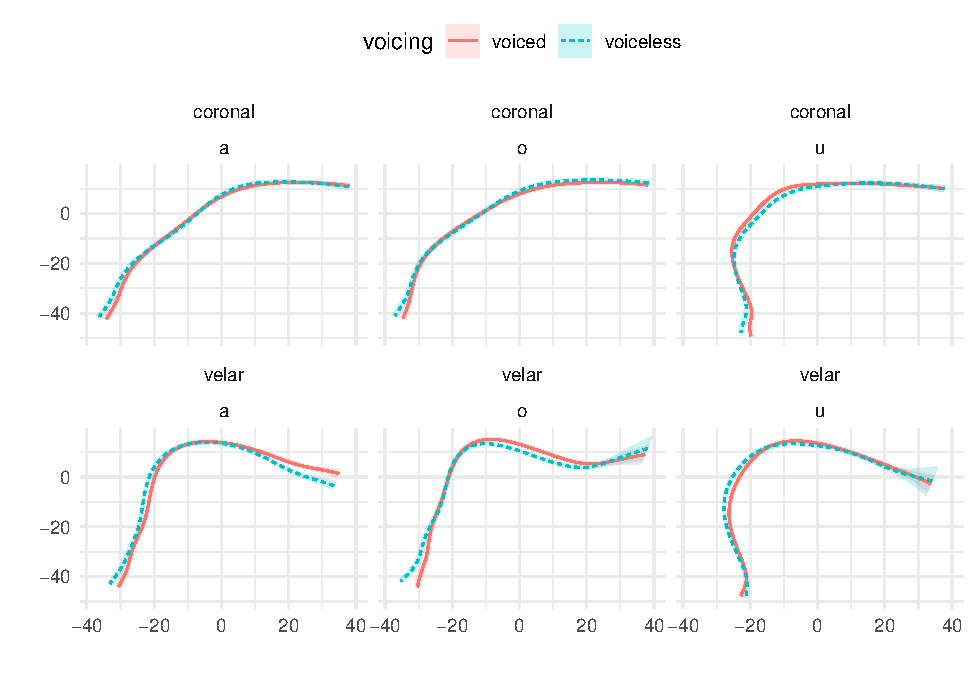
\includegraphics[width=.8\textwidth]{2018-polar-gam_files/figure-latex/Figure07} 

}

\caption{Tongue contours of voiceless and voiced stops in IT01.}\label{f:Figure07}
\end{figure}

\begin{figure}

{\centering 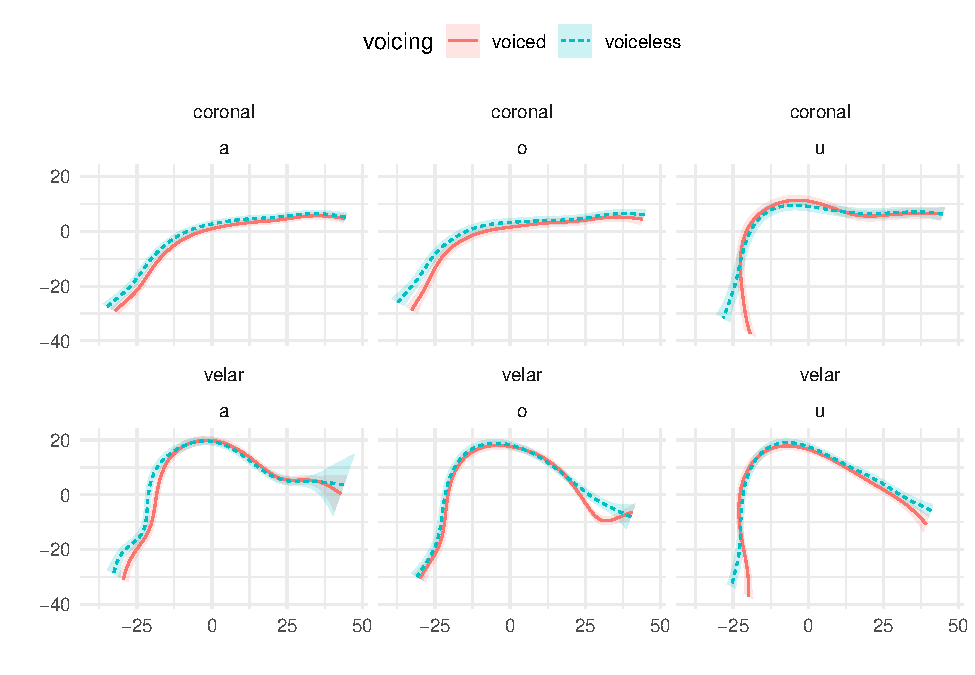
\includegraphics[width=.8\textwidth]{2018-polar-gam_files/figure-latex/Figure08} 

}

\caption{Tongue contours of voiceless and voiced stops in IT02.}\label{f:Figure08}
\end{figure}

\begin{figure}

{\centering 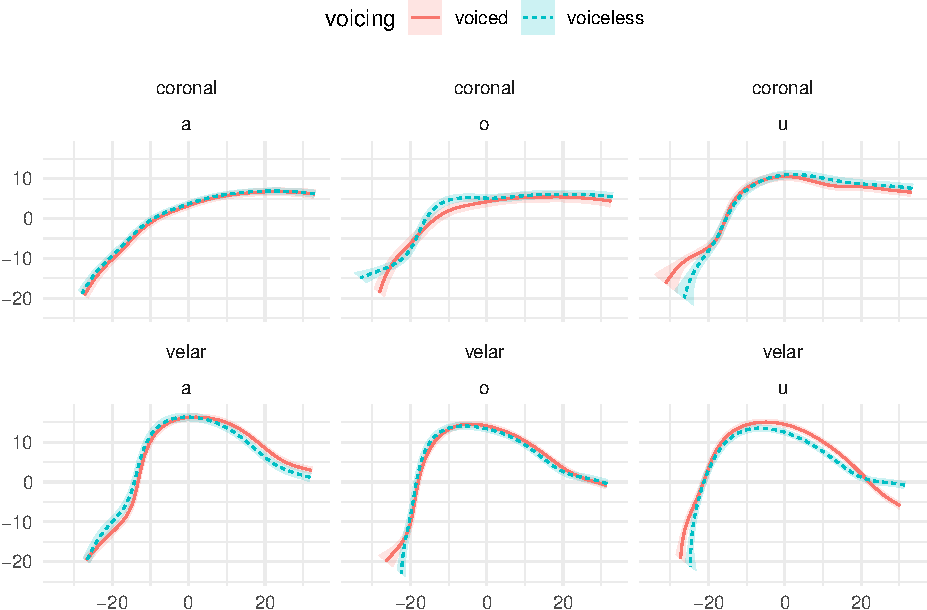
\includegraphics[width=.8\textwidth]{2018-polar-gam_files/figure-latex/Figure09} 

}

\caption{Tongue contours of voiceless and voiced stops in IT03.}\label{f:Figure09}
\end{figure}

\begin{figure}

{\centering 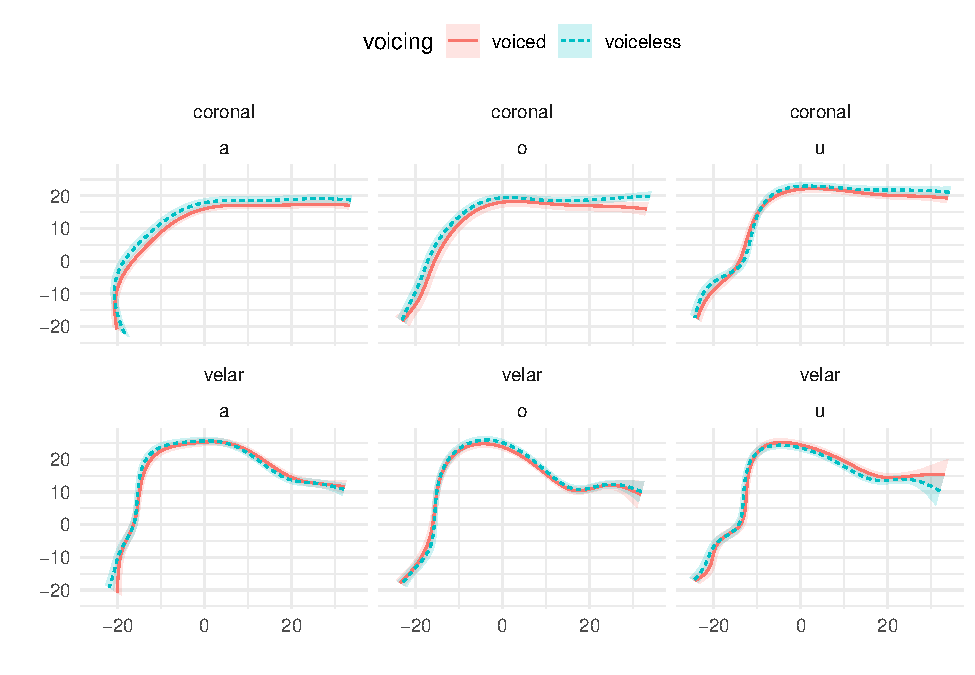
\includegraphics[width=.8\textwidth]{2018-polar-gam_files/figure-latex/Figure10} 

}

\caption{Tongue contours of voiceless and voiced stops in IT04.}\label{f:Figure10}
\end{figure}

\begin{figure}

{\centering 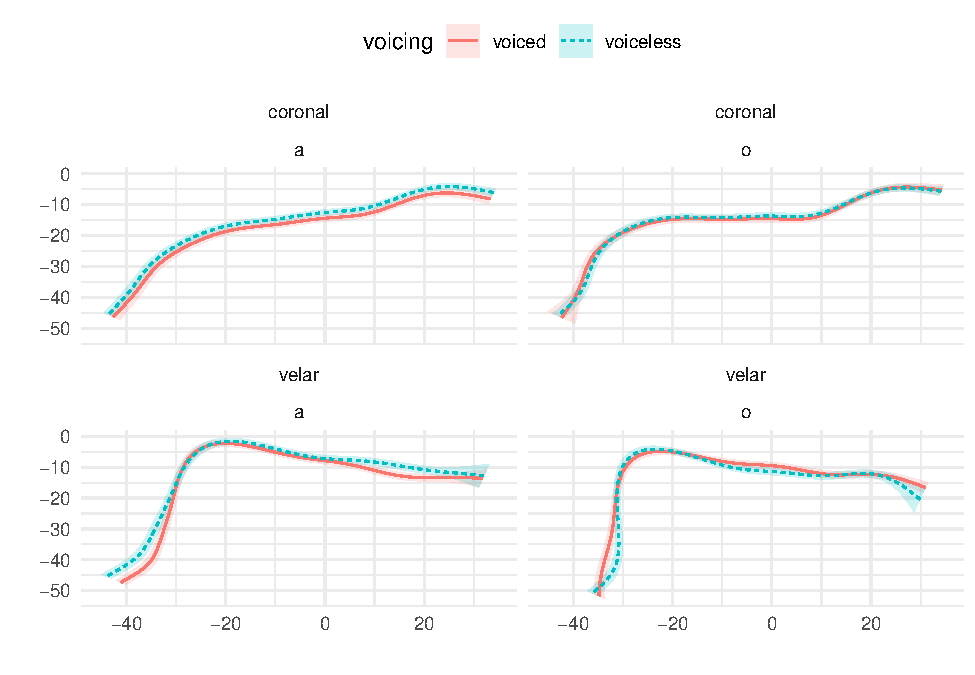
\includegraphics[width=.8\textwidth]{2018-polar-gam_files/figure-latex/Figure11} 

}

\caption{Tongue contours of voiceless and voiced stops in IT07.}\label{f:Figure11}
\end{figure}

\begin{figure}

{\centering 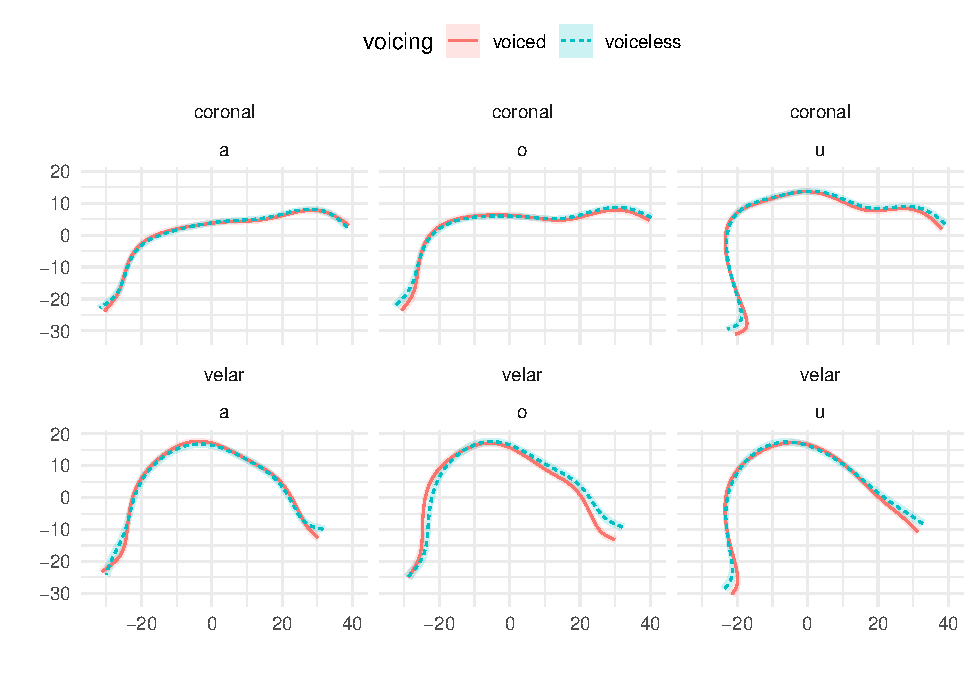
\includegraphics[width=.8\textwidth]{2018-polar-gam_files/figure-latex/Figure12} 

}

\caption{Tongue contours of voiceless and voiced stops in IT11.}\label{f:Figure12}
\end{figure}

\begin{figure}

{\centering 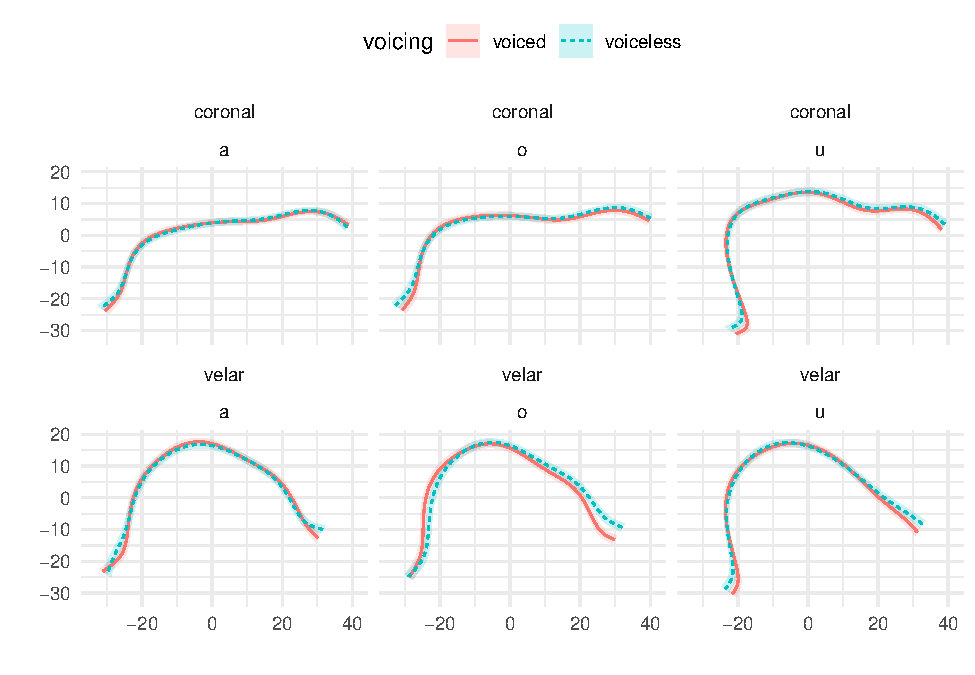
\includegraphics[width=.8\textwidth]{2018-polar-gam_files/figure-latex/Figure13} 

}

\caption{Tongue contours of voiceless and voiced stops in PL02.}\label{f:Figure13}
\end{figure}

\begin{figure}

{\centering 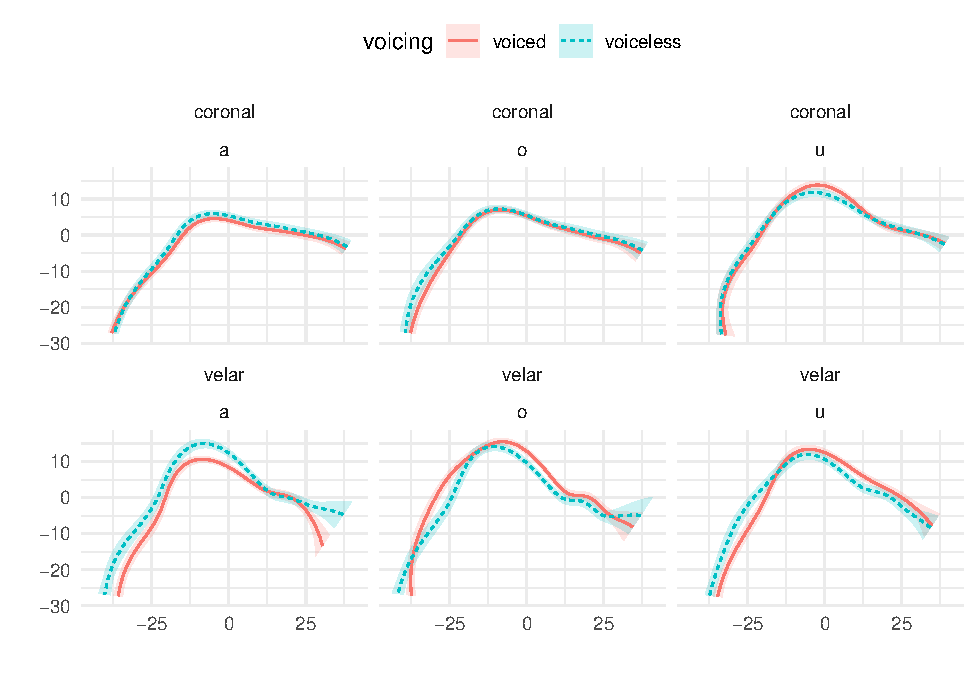
\includegraphics[width=.8\textwidth]{2018-polar-gam_files/figure-latex/Figure14} 

}

\caption{Tongue contours of voiceless and voiced stops in PL03.}\label{f:Figure14}
\end{figure}

\begin{figure}

{\centering 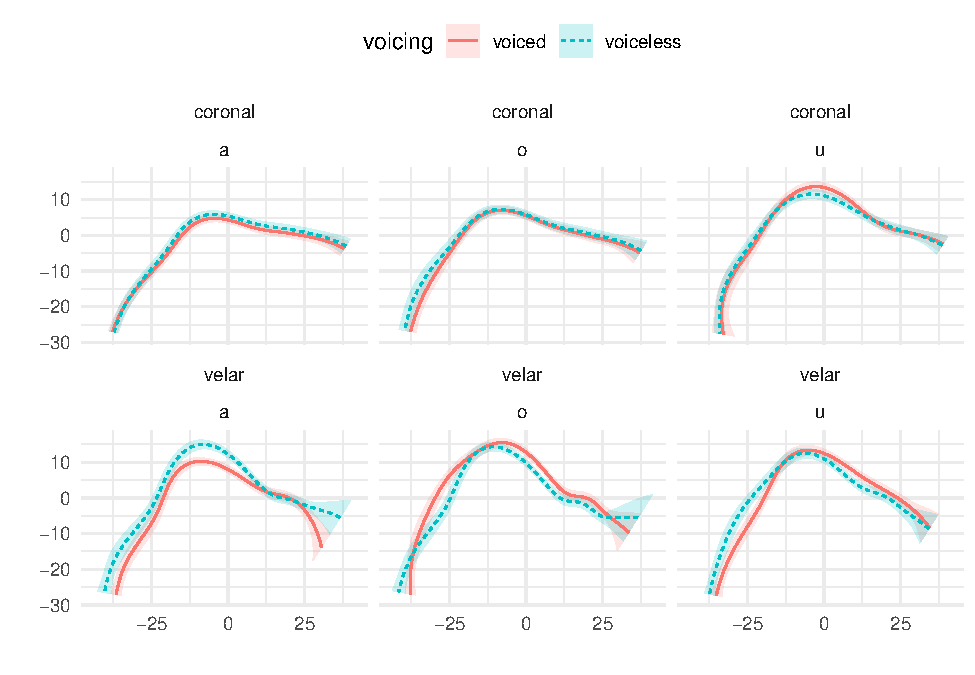
\includegraphics[width=.8\textwidth]{2018-polar-gam_files/figure-latex/Figure15} 

}

\caption{Tongue contours of voiceless and voiced stops in PL04.}\label{f:Figure15}
\end{figure}

\begin{figure}

{\centering 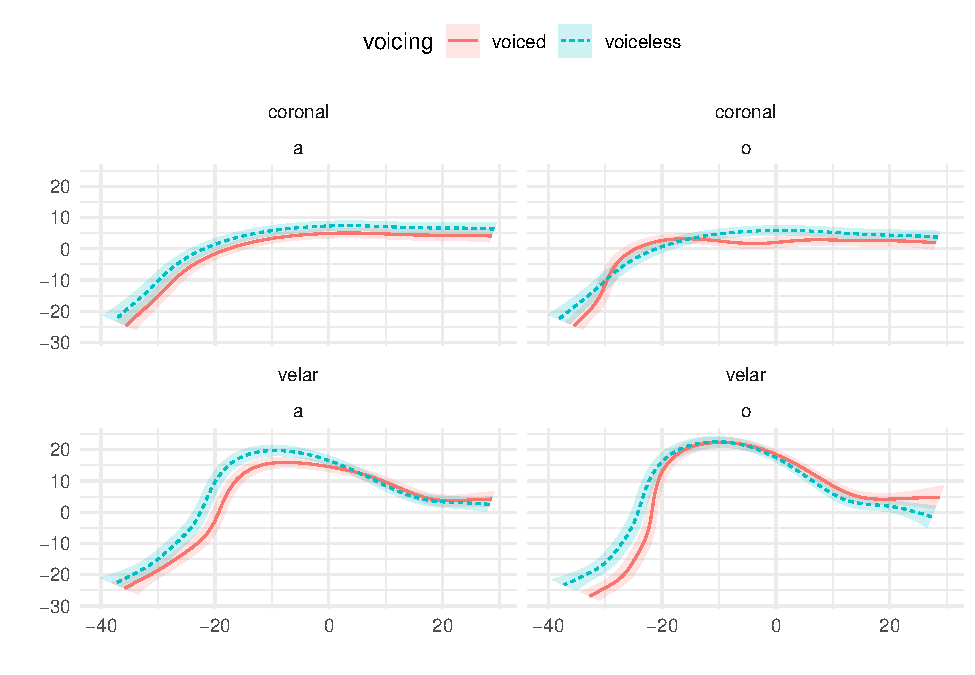
\includegraphics[width=.8\textwidth]{2018-polar-gam_files/figure-latex/Figure16} 

}

\caption{Tongue contours of voiceless and voiced stops in PL05.}\label{f:Figure16}
\end{figure}

\begin{figure}

{\centering 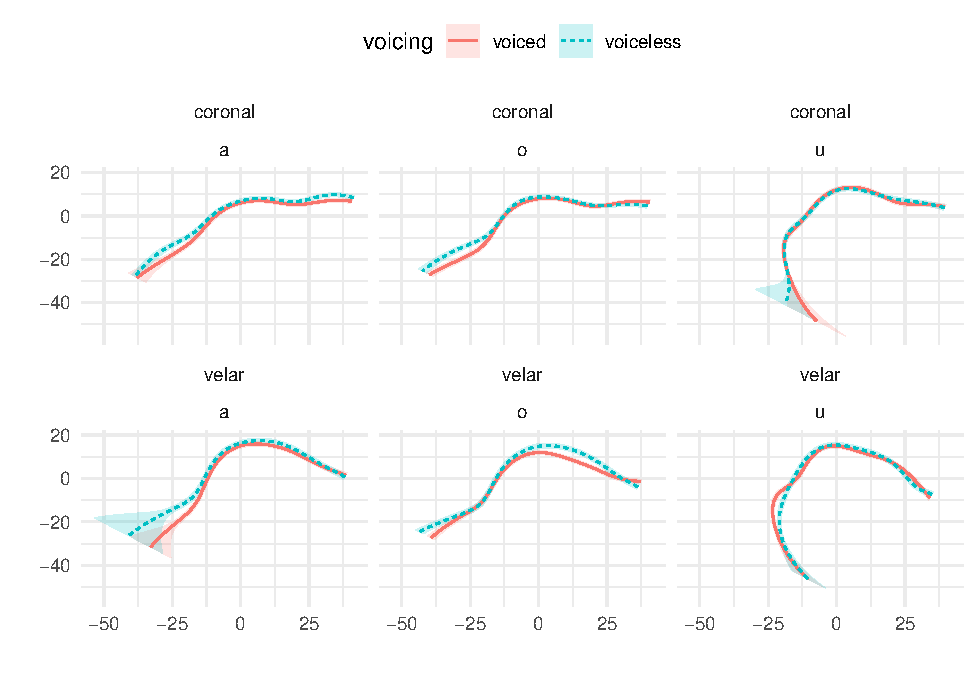
\includegraphics[width=.8\textwidth]{2018-polar-gam_files/figure-latex/Figure17} 

}

\caption{Tongue contours of voiceless and voiced stops in PL06.}\label{f:Figure17}
\end{figure}

\begin{figure}

{\centering 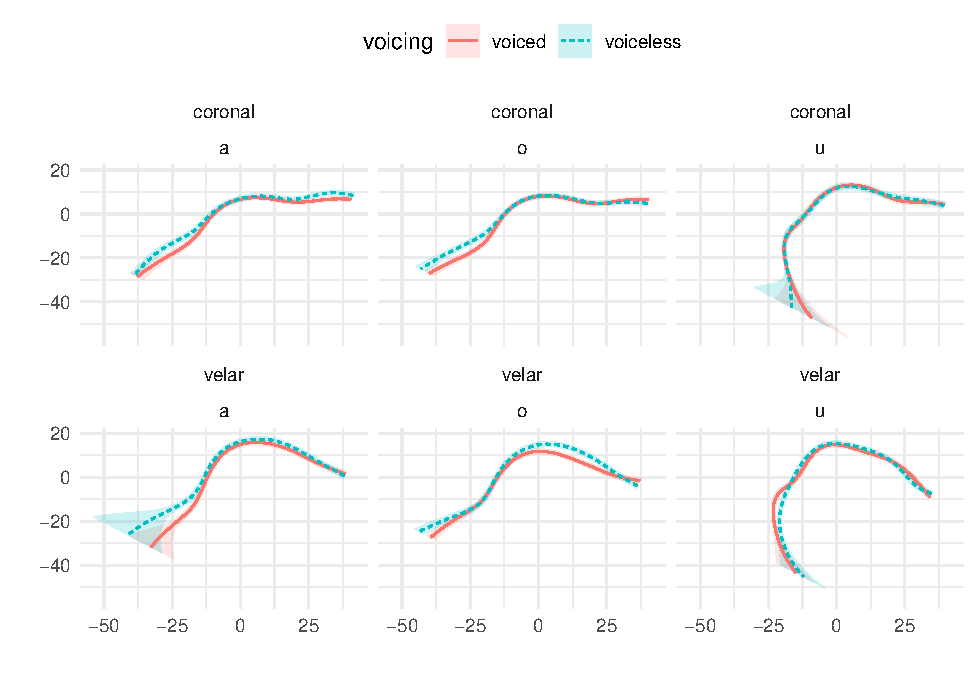
\includegraphics[width=.8\textwidth]{2018-polar-gam_files/figure-latex/Figure18} 

}

\caption{Tongue contours of voiceless and voiced stops in PL07.}\label{f:Figure18}
\end{figure}

\hypertarget{conclusions}{%
\section{Conclusions}\label{conclusions}}

Generalised additive (mixed) models (GAMs) can be efficiently used to
statistically assess differences in tongue contour shapes as obtained
from ultrasound tongue imaging. This paper showed how GAMs can be fitted
to tongue contours in polar coordinates in R with the specialised
package rticulate. An example of how GAMs can help modelling differences
in tongue contours has been illustrated with data from 12 speakers of
Italian and Polish in which the mid-sagittal tongue contours of
voiceless and voiced stops where compared. The advantages of polar GAMs
over the current implementation of polar tongue SSANOVA include: the
ability to specify multiple predictors and random effects; control over
the autocorrelation in the residuals which could otherwise make the
model overconfident; separate methods for assessing statistical
significance at the level of the predictor (with model comparison) and
for identifying which part of the tongue differs significantly (by
visualising the difference smooths). The same general issues noted in
\citet{davidson2006} for SSANOVA apply to polar GAMs. In particular,
while within-speaker normalisation can be achieved by rotation and
offsetting of the data relative to a bite plate (as done here),
across-speaker normalisation represents a bigger challenge. Since we
can't be deduced with sufficient certainty from the ultrasonic image
which part of the tongue is being actually imaged, it is not possible to
define fixed anatomical landmarks across speakers that can be used in
normalisation. For this reason it has been recommended here to fit
separate models for each speaker. Future work will explore ways of
allowing the user to use data aggregated from multiple speakers while
accounting for the uncertainty in which parts of the tongue are imaged.
Finally, polar GAMs can also be readily extended to model 3D tongue
surfaces and whole tongue contours differences over time (in other
words, how the sectional shape of the tongue changes over time).

\hypertarget{data-accessibility-statement}{%
\section{Data Accessibility
Statement}\label{data-accessibility-statement}}

The data and code used in this paper can be viewed and downloaded at the
Open Science Framework link
\url{https://osf.io/q7hyz/?view_only=f9d9f865619848f4bc575bc86cb07282}.

\bibliography{linguistics.bib}


\end{document}
